%!TEX root = /Users/Nikolaj/Developer/GPU-Project/Report/Report.tex
To make sure that the C\#, C and CUDA programs produce similar results up to an acceptable threshold, we run each program on a large data set and compare the outputs. Each of the 3 programs take 4 command line arguments which is (1) \emph{g} - the number of years from the policyholder dies until the first rate is disbursed, (2) \emph{r} -  age of retirement, (3) \emph{x} age at runtime and (4) \emph{stepsize} - the number of steps to take each year when the outer and the inner models are solved. Each program outputs a single number which is INSERT DESCRIPTION. \\

We want all input from the test data set to fall within intervals that are chosen realistically and individually for each command line argument. It makes little sense to test the 3 programs with a retirement age of 200 since few people experience to become that old. Likewise, a big stepsize will make the overall test take very long time to complete which is impractical when testing during development. To avoid these problems, we made a program that generates test data in the shape of a plain text file. Each row in the file contains a comma separated list of numbers representing the 4 command line arguments to be fed to each of the 3 programs. \\

Next, we need a program that reads the lines of the test data file one by one, invokes the 3 programs in sequence and writes the corresponding results to a line in a new file. Obviously, this could be done by a single program as just described, but we wish to be able to test the C\#, C and CUDA programs separately during development without having to wait for the other 2 to finish, which might take longer time than the single program we want to test. For that reason, we make a test program for each of the 3 programs that reads a line from the test data file, invokes the program and appends the result to a text file that is private to the program being tested. \\

Finally, we have 3 text files with the results from each test run. We can then import the contents of each file into a column in a spread sheet and have the sheet compare the numbers on each row to identify matching and differing results. \\

The test scenario describe above was conducted on 3 machines with the following hardware specifications

\begin{table}
\begin{center}
\begin{tabular}{|c|c|c|}
	\hline
	\multicolumn{1}{|m{2.8cm}|}{\centering \textbf{Machine}} & The Malamanteau server & Desktop PC1 \\ \hline
	\multicolumn{1}{|m{2.8cm}|}{\centering \textbf{OS}} & Windows 7 Pro 64-bit & Windows 7 Pro 64-bit\\ \hline
	\multicolumn{1}{|m{2.8cm}|}{\centering \textbf{CPU}} & Intel Xeon W3505 2.53 GHz & Intel Core i7-940 2.92 GHz \\ \hline
	\multicolumn{1}{|m{2.8cm}|}{\centering \textbf{RAM}} & 4 GB & 12 GB DDR3\\ \hline
	\multicolumn{1}{|m{2.8cm}|}{\centering \textbf{GPU}} & Nvidia Tesla C2075\cite{tesl} & Nvidia GeForce GTX 295 \cite{gtxx}\\ \hline
	\multicolumn{1}{|m{2.8cm}|}{\centering \textbf{CC}} & 2.0 & 1.3\\ \hline
	\multicolumn{1}{|m{2.8cm}|}{\centering \textbf{CUDA cores}} & 448 & 480\\ \hline
	\multicolumn{1}{|m{2.8cm}|}{\centering \textbf{Frequency of CUDA cores}} & 1.15 GHz & Unknown\\ \hline
	\multicolumn{1}{|m{2.8cm}|}{\centering \textbf{Total dedicated memory}} & 6 GB GDDR5 & 1792 MB GDDR3\\ \hline
\end{tabular}
\end{center}
\caption{Test machines part 1}
\end{table}

\begin{table}
\begin{center}
\begin{tabular}{|c|c|}
	\hline
	\multicolumn{1}{|m{2.8cm}|}{\centering \textbf{Machine}} & Gpulab06 \\ \hline
	\multicolumn{1}{|m{2.8cm}|}{\centering \textbf{OS}} & UNIX \\ \hline
	\multicolumn{1}{|m{2.8cm}|}{\centering \textbf{CPU}} & Intel Core i7-3820 3.60GHz \\ \hline
	\multicolumn{1}{|m{2.8cm}|}{\centering \textbf{RAM}} & 32 GB \\ \hline
	\multicolumn{1}{|m{2.8cm}|}{\centering \textbf{GPU}} & NVIDIA Tesla K20c (INDSÆT REF) \\ \hline
	\multicolumn{1}{|m{2.8cm}|}{\centering \textbf{CC}} & 3.5 \\ \hline
	\multicolumn{1}{|m{2.8cm}|}{\centering \textbf{CUDA cores}} & 2496 \\ \hline
	\multicolumn{1}{|m{2.8cm}|}{\centering \textbf{Frequency of CUDA cores}} & Unknown \\ \hline
	\multicolumn{1}{|m{2.8cm}|}{\centering \textbf{Total dedicated memory}} & 5 GB GDDR5 \\ \hline
\end{tabular}
\end{center}
\caption{Test machines part 1}
\end{table}

For testing purposes we assume that the insurance holder is always a woman and the spouse is always a man. The individual test results kan be found in INDSÆT APPENDIX ELLER CD REF.

\begin{figure}
\begin{center}
	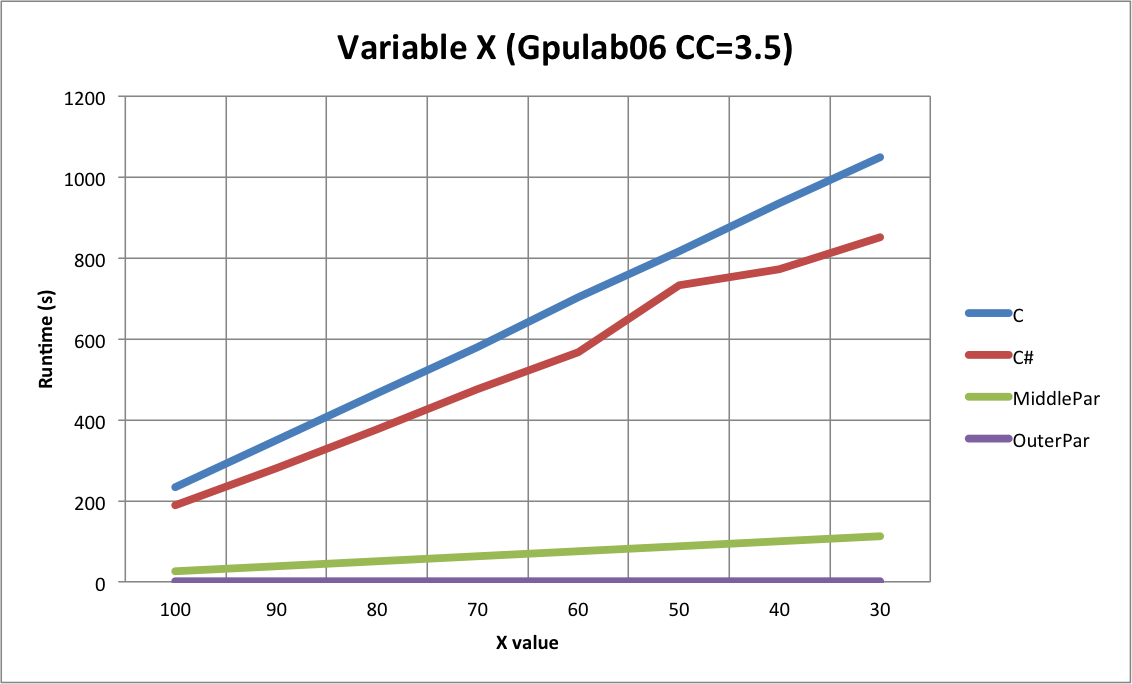
\includegraphics[width=\textwidth]{img/Gpulab-varx35.png}
\end{center}
\caption{The impact of changing the $x$ value on the Gpulab06 machine}
\end{figure}

